\documentclass{article}
\usepackage[letterpaper]{geometry}
\usepackage[utf8]{inputenc}
\usepackage{amsmath}
\usepackage{amssymb}
\usepackage{xcolor}
\usepackage{natbib}
\usepackage{graphicx}
\newcommand{\red}[1]{\textcolor{red}{#1}}
\newcommand{\blue}[1]{\textcolor{blue}{#1}}
\newcommand{\gray}[1]{\textcolor{gray}{#1}}
\newcommand{\green}[1]{\textcolor{green}{#1}}
\newcommand{\mat}[1]{\boldsymbol{\mathsf{#1}}}
\renewcommand{\vec}[1]{\boldsymbol{\mathrm{#1}}}
\newcommand{\R}[1]{\mathbb{R}^{#1}}
\bibliographystyle{unsrtnat}
\title{Learning Nonlinear Dynamics Using Kalman Smoothing}
\author{Jake Stevens-Haas$^*$, Yash Bhangale$^*$, J. Nathan Kutz$^{*,\dag}$, Aleksander Aravkin$^*$\\
{\small $^*$Department of Applied Mathematics, University of Washington, Seattle, WA} \\
{\small $^\dag$ Department of Electrical and Computer Engineering, University of Washington, Seattle, WA} }
\date{\today}

\begin{document}

\maketitle

\abstract{Identifying Ordinary Differential Equations (ODEs) from measurement data requires both fitting the dynamics and assimilating, either implicitly or explicitly, the measurement data.
The Sparse Identification of Nonlinear Dynamics (SINDy) method involves a derivative estimation step (and optionally, smoothing) and a sparse regression on a library of candidate ODE terms.
Kalman smoothing is a classical framework for assimilating the measurement data whose noise behavior is well understood.
Previously, derivatives in SINDy and its python package, pysindy, had been estimated by finite difference, L1 total variation minimization, or local filters like Savitsky-Golay.
In contrast, Kalman discovers ODEs that best recreate the essential dynamics in simulation versus \green{compare to commonly used metrics}, and when combined with hyper-parameter optimization, requires the least amount of tuning.
We have incorporated Kalman smoothing into the existing pysindy architecture, allowing for rapid adoption of the method.
Kalman smoothing appears to be the most amenable to parameter selection and best at preserving problem structure in the presence of noise.
This is demonstrated on a number of dynamical systems.}

\section{Introduction}
The method of {\em Sparse Identification of Nonlinear Dynamics} (SINDy)~\cite{Brunton2016,brunton2022data} seeks to discover a differential or partial differential equation governing an arbitrary, temporally measured system.
The method takes as input some coordinate measurements over time, such as angles between molecular bonds~\cite{Boninsegna2018} or a spatial field, such as wave heights~\cite{Rudy2017}, and returns the best ordinary or partial differential equation (ODE or PDE) from a library of candidate terms.
However, the method struggles to accommodate significant measurement noise.
On the other hand, Kalman theory has a half-century history of assimilating measurement noise to smooth a trajectory, with well-studied and rigorously characterized noise properties.
We integrate the mature and well-established theory of Kalman with the emerging SINDy technology and combine with generalized cross validation parameter selection for systematic practical applications.
Our Kalman SINDy architecture is shown to be competitive with other combinations of data smoothing and system identification techniques, and has a significant advantage in preservation of problem structure and ease of parameter selection.
However, the method struggles to accomodate significant measurement noise.
On the other hand, Kalman theory has a half-century history of assimilating noisy data to smooth a trajectory.
Its noise properties have been well studied.
The paper integrates mature, well-established Kalman theory with emerging SINDy technology and generalized cross validation parameter selection.
It finds that the combination is competitive with other combinations of data smoothing and system identification, and has an advantage in preservation of problem structure and ease of parameter selection.

% \begin{itemize}
%     \item Model discovery in data science - bring power of kalman here (what about other methods: autoencoders, DMD, Koopman) (what for?) (All of physics specifying relationships among derivatives) (your job is to discovery derivatives, because derivatives give you the models. There's a lot more we can say, study, and understand about a system when we can identify relationships between derivatives.
%     \item SINDy - overview (2016 + )
%     \item Kalman overview (citing textbooks: Kalman is (a) Euler update, (b) Filter update with normal random variable, (c) MLE of Brownian motion, (d) best linear fit) engineering practice and design have used it for control, data assimilation is used as a workhorse tool in the real world e.g. weather.  Plus Auto KS  Include words from https://www.sciencedirect.com/science/article/pii/S0003267000838398 about comparison between SG and Kalman.  Include words from https://en.wikipedia.org/wiki/Local\_regression about comparison between SG and LOES.
%     \item What we do: marriage of kalman + SINDy (figure, hinted at in P1)
% \end{itemize}

Model discovery methods are emerging as a critical component in data-driven engineering design and scientific discovery.
Enabled by advancements in computational power, optimization schemes, and machine learning algorithms, such techniques are revolutionizing what can be achieved from sensor measurements deployed in a given system.
Of interest here is the discovery of dynamic models, which can be constructed from a diversity of techniques, including simple regression techniques such as the {\em dynamic mode decomposition} (DMD)~\cite{kutz2016dynamic,ichinaga2024pydmd} to neural networks such as {\em physics-informed neural networks} (PINNs)~\cite{Raissi2019}.
In such models, the objective is to construct a proxy model for the observed measurements which an be used to characterize and reconstruct solutions.
While DMD provides an interpretable model in terms of a modal decomposition, most neural network architectures remain black-box without a clear view of the underlying dynamical processes.
Although the number of techniques available are beyond the scope of this paper to review~\cite{cuomo2022scientific}, SINDy is perhaps the leading data-driven model discovery method for interpretable and/or explainable dynamic models as it looks to infer the governing equations underlying the observed data.
As such, it looks to construct a model in terms of relationships between spatial and/or temporal derivatives, which is the underlying mathematical representation of physics and engineering based systems since the time of Newton.

The SINDy regression architecture seeks to robustly establish relationships between derivatives.
Emerging from~\cite{Brunton2016,brunton2022data}, all variants aim to discover a sparse symbolic representation of an autonomous or controlled system, $\dot x = f(x)$.
A diversity of methodological innovations have been introduced into the SINDy discovery framework to make it robust and stable, including the \emph{weak form} optimization by Messenger and Bortz~\cite{messenger2021bweak,messenger2021weak}.
This approach solves the sparse regression problem after integrating the data over random control volumes, providing a dramatic improvement to the noise robustness of the algorithm.
Weak form optimization may be thought of as a generalization of the integral SINDy~\cite{Schaeffer2017} to PDE-FIND.
Further improvements to noise robustness and limited data may be obtained through ensembling techniques~\cite{Fasel2022}, which use robust statistical bagging and are equivalent to Bayesian inference~\cite{gao2022bayesian,gao2023convergence}, to learn inclusion probabilities for the sparse terms $\xi$ from limited and noisy data.
These methodological innovations are integrated in the open-source PySINDy software library~\cite{Kaptanoglu2022}, reducing the barrier to entry when applying these methods to new problems.  Additional techniques for learning dynamics from data include PDE-NET~\cite{Long2019,Long2018} and the Bayesian PDE discovery from data~\red{atkinson2020bayesian}.
Symbolic learning has also been developed, including symbolic learning on graph neural networks~\red{cranmer2019learning,cranmer2020discovering,sanchez2020learning}.

Kalman smoothing, which this paper adds to SINDy, has a long history of assimilating measurement data in time series.
From its debut in~\cite{kalman, KalBuc}, engineering practice and design have used it for control and prediction across the real world, e.g. in radar systems, econometric variables, weather prediction, and more.
The family of Kalman methods encompasses both smoothing, after-the-fact techniques, and filtering, real-time updates, that derive from the same assumptions for distributions.
The Kalman smoother can be considered as a best-fit Euler update, the maximum likelihood estimator of Brownian motion, or as the best linear fit of an unknown system.
The best fit/maximum likelihood view extends the classic Kalman updates to a rich family of efficient generalized Kalman smooth algorithms for signals corrupted by outliers, nonlinear models, constraints through side information, and a myriad of other applications~\cite{aravkin2017generalized}.
In the simplest invocation, the Kalman estimator is determined given only the ratio of measurement noise to the process's underlying stochastic noise.
Fixing both of these parameters allows Kalman methods to also identify the variance of the associated estimator.
Furthermore, much work exists to attempt to identify parameters purely from data, such as \cite{Barratt2020,VanBreugel2020}.
These methods include their own parameters and are not guaranteed a solution, but are an improvement on the indeterminate nature of direct maximum likelihood or MAP likelihood.

This paper introduces Kalman smoothing as the derivative estimation step in SINDy in distinction with the L1 total variation minimization or Savitsky-Golay smoothers common in application.
By introducing a continuous process loss for derivative estimation, it begins to reconcile the derivative estimation step to the symbolic regression step in a principled manner.
It allows engineering applications to incorporate SINDy estimation with a familiar data assimilation technique whose noise properties are well understood.

Section two describes the individual methods of SINDy and Kalman smoothing, providing some literature review.  In section three, experiments demonstrate the advantages of incorporating Kalman with SINDy.  The paper concludes with avenues for future research in section four.

\section{Background}

\subsection{SINDy}
SINDy \cite{Brunton2016} is a family of emerging methods for discovering the underlying dynamics of a system governed by unknown or partially-known \cite{Champion2020} differential equations.  It can handle ODEs as well as PDEs \cite{Rudy2017}, and has been used for protein folding \cite{Boninsegna2018}, chemical reaction networks \cite{Hoffmann2019}, plasma physics \cite{Guan2021}, and more.  Most invocations occur through the pysindy Python package, but innovations such as Langevin Regression \cite{Callaham2021} or \cite{Rudy2019} exist as independent code.

\begin{figure}[ht]
    \label{fig:sindy}
    \centering
    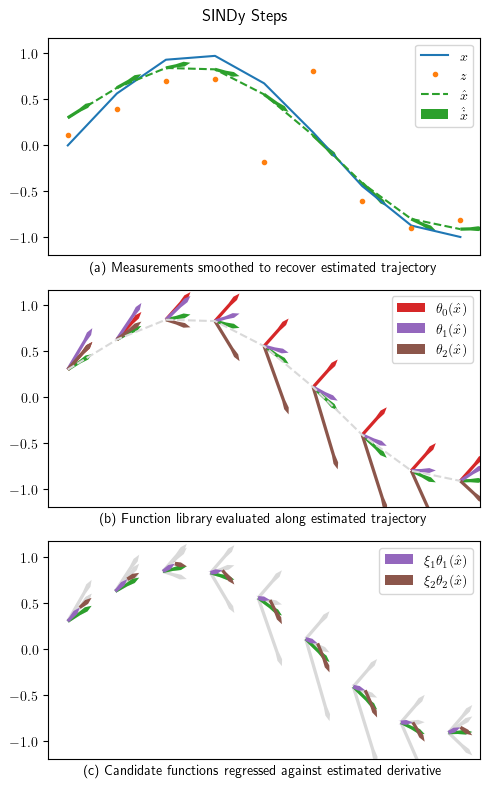
\includegraphics[width=.5\textwidth]{images/explain_sindy}
    \caption{The SINDy method, applied to fitting a sinusoid.  Taking noisy data, it identifies the model $\dot x = \xi_1\theta_1(x) + \xi_2\theta_2(x)$, rejecting $\theta_0$.}
\end{figure}


Given some variable of interest $\mat X$ and a library of functions $\mat \Theta$ (including spatial derivatives, when relevant) SINDy seeks to find the coefficients $\mat \Xi$ of the differential equation:

\begin{align}
    \label{eqn:sindy_ode}
    \dot X = \Xi\Theta(X)
\end{align}

To amplify:
\begin{align*}
    &\mat X \in \R{n \times m}\text{: system of $n$ coordinates at $m$ timepoints.}\\
    &\mat \Theta(X) \in \R{p \times m}\text{: library of $p$ functions evaluated at $m$ timepoints}\\
    &\mat \Xi \in \R{n \times p}\text{: coefficients for $n$ equations of $p$ functions}
\end{align*}
The function library written as a time-independent quantity refers to the collection $\mat \Theta = [\theta_1, \dots \theta_p]^T$, where $\theta_i: \R{n}\rightarrow\R{}$. Examples include the family of all degree-2 polynomials of $n$ inputs, mixed sines and cosines of certain frequencies, or any user-specified family.

The method generally proceeds in two steps:

\begin{enumerate}
    \item Estimate the time derivatives of the system ${\mat{\widehat{\dot X}}} = G(\mat X)$ for some smoothing function $G$
    \item Choosing a sparse regression method, solve the problem $\underset{\text{sparse } \mat \Xi}{\arg\min} \left\| \mat{\widehat{\dot{X}}} - \mat \Xi \mat \Theta(\mat X) \right\|^2$
\end{enumerate}
This general process is sketched out in Figure \ref{fig:sindy}.  Researchers have tried a few different methods for calculating the derivatives, broadly grouped into  global methods (e.g. L-1 total variation minimization of \cite{Chartrand2011}) and local methods (e.g. Savitsky-Golay smoothing).  Different ways of applying sparsity has attracted more attention, including sequentially thresholding linear regression, a direct L-0 penalty \cite{Champion2020}, an L-0 constraint \cite{Bertsimas2023}, and bayesian methods for a prior distribution such as spike-slab or regularized horseshoe priors \cite{Hirsh2022,gao2022bayesian}.  Those two papers also demonstrate an interesting line of innovation, eschewing derivatives and using the integral of function library in the loss term.  A related approach instead uses the weak form of the differential equation, yielding a solution that {\it is} convex, but which does not provide as straightforwards an interpretation of the measurement noise. \blue{Verify this}  Most of these methods can benefit from ensembling the data and library terms, as in \cite{Fasel2022}, but others, such as \cite{Kaptanoglu2021} for identifying Galerkin modes of globally stable fluid flows, require a specific form of function library.

% A trade-off SINDy faces is that while sparse regression techniques work better with orthogonal basis functions, ODE for most physical systems have terms that are not orthogonal, e.g. the Lorenz system.

This paper seeks to make SINDy more resilient to noise by taking a data assimilation approach.  It instead presents the Kalman SINDy steps
\begin{enumerate}
    \item Estimate the state and time derivatives of the system ${\mat{\widehat{\dot X}}}, \mat{\widehat X} = G(\mat X)$ where $G$ applies Kalman smoothing
    \item Choosing a sparse regression method, solve the problem $\underset{\text{sparse } \mat \Xi}{\arg\min} \left\| \mat{\widehat{\dot{X}}} - \mat \Xi \mat \Theta(\mat {\widehat X}) \right\|^2$
\end{enumerate}

\subsection{Kalman Smoothing}

Kalman filtering and smoothing refers to a group of optimal estimation techniques to assimilate measurement noise to a random process.
Filtering refers to incorporating  new measurements in real-time, while smoothing refers to estimating the underlying state or signal using a complete trajectory of (batch) measurements.
While the processes this paper is concerned with are not random, in the first step of SINDy they are unknown, and so probabilistic language is appropriate.

In adding Kalman smoothing to SINDy, we introduce a distinction between the measurement variables and the state variables of the dynamical system in equation
\ref{eqn:sindy_ode}.  As such, the inputs to the problem become $m$ time points of measurements of $k$ variables ($\mat Z\in \R{k\times m}$) and a linear transform from the state to the measurement variables $\mat H \in \R{n \times k}$ describing how the process is measured.

Measurement error is assumed to be normally distributed with $\mat H \mat X - \mat Z \sim \sigma_z \mathcal N(0, \mat R)$ where the covariance matrix $\mat R\in\R{k \times k}$.  Measurement regimes where noise is autocorrelated or varies over time can be accomodated by flattening $\mat H \mat X - \mat Z$ and describing $\mat R\in\R{nk \times nk}$.

Two parameters are required $\sigma_z$, the measurement noise standard deviation, and $\sigma_x$, the process velocity standard deviation per unit time.  If only point estimates of the state, and not variances of those estimates, are required, it suffices to use the ratio $\rho = (\sigma_z / \sigma_x)^2$.

\begin{figure}
    \label{fig:kalman}
    \centering
    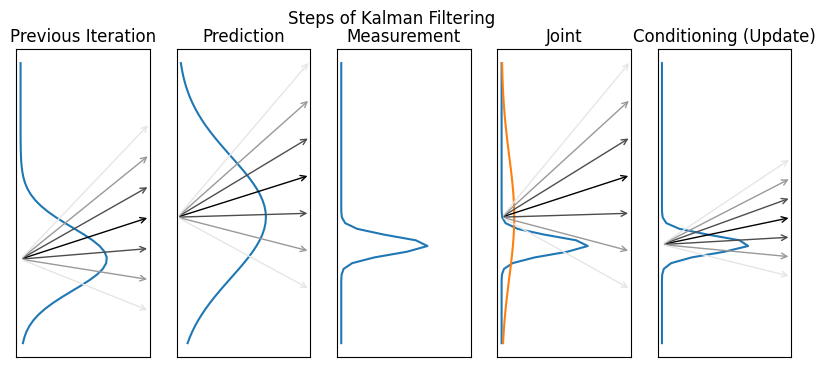
\includegraphics[width=\textwidth]{images/static/kalman_fit_demo2.png}
    \caption{Explanatory depiction of Kalman filtering.
    A previous iteration gives a distribution $p(x_{i-1},\dot x_{i-1})$.
    Multiplication by an update matrix produces the predictions $p(x_i, \dot x_i|x_{i-1}, \dot x_{i-1})$.
    Simultaneously, measurements $z_i$ are taken that, with known measurement noise, give $p(z_i|x_i)$.
    Multiplication gives the joint distribution $p(x_i, \dot x_i, z_i| x_{i-1}, \dot x_{i-1})$, from which the conditional distribution $p(x_i, \dot x_i|z_i, x_{i-1}, \dot x_{i-1})$ can be calculated, shown in \cite{Eaton2007}}
\end{figure}


Each process is assumed to have an independent, Brownian velocity.  This leads to Kalman smoothing estimator:
\begin{align}
    \underset{X, \dot X}{\arg\min}{\|\mat H \mat X - \mat Z\|_{\mat R^{-1}}}^2 + \rho {\|\mat G [\mat {\dot X}, \mat X]\|_{\mat Q^{-1}}}^2
\end{align}
Here, $\mat G$ is a linear transform to separate $[\mat{\dot X}, \mat X]$ into independent, mean-zero increments, and $\mat Q$ is the covariance of the Brownian process velocity $\mat{\dot X}$ and its integral, $\mat X$ over the increments.  A graphic displaying Kalman filtering is shown in Figure \ref{fig:kalman}.  Although this paper uses global smoothing, the equivalent step-by-step approach of filtering is more amenable to graphics

In practice, rather than choosing $\rho$, this paper uses the generalized cross validation of \cite{Barratt2020} to choose $\rho$.  It chooses $\rho$ in order to minimize the loss on a witheld set of data.  While the algorithm described in that paper is not guaranteed to find a minimum, heuristic experience has shown that the longer the trajectory, the more likely their algorithm will succeed.  As the experiments in the next section use simulated data, this limitation is acceptable.

The generalized cross validation approach of \cite{Barratt2020} witholds some measurement points in order to find the values of $\mat H, \mat R, \mat G,$ and $\mat Q$ that produce estimates $\hat{\mat X}$ that fit witheld data most accurately.  This powerful approach can apply to all linear systems but comes with the burdens of nonconvexity.  In our work, we presume to know the measurement parameters and most of the process parameters - after all, "position is the integral of velocity", implies certain constraints on $\mat G$ and $\mat Q$.  The method accomodates these constraints via specification of a prox function.

\begin{itemize}
    \item \blue{Anything on existing Kalman System Identification?}
\end{itemize}

\section{Experiments}

We seek to evaluate the value of Kalman smoothing as a step in SINDy in comparison to other noise-mitigation innovations.  We simulate seven canonical dynamical systems with noisy measurements across a variety of initial conditions, discovering ODEs from SINDy approaches with different smoothing methods.  To compare the methods, we then integrate the discovered equations and observe how well they preserve the system's structure as well as directly comparing the coefficients through the F1 score and mean absolute error (MAE).

We compare the results of SINDy with Kalman smoothing and the hyperparameter optimization of \cite{Barratt2020} in comparison with alternative smoothing methods: L-1 total variation minimization and Savitsky-Golay.  The latter smoothing methods have been modified to pass the not just the smoothed derivatives $\mat{\widehat{\dot X}}$, but also the smoothed position estimates $\mat {\widehat X}$ to the second step of SINDy.  They also each require a parameter: TV requires a coefficient for the L-1 regularizer and Savitsky-Golay requires a smoothing window.  These are gridsearched over a wide range, although it is worth noting that choosing the gridsearched optimum requires knowledge of the true system, in distinction to the method used for Kalman smoothing.

Beyond the differentiation step, the SINDy models also specify a function library and optimizer.  The feature library used for all experiments was cubic polynomials, including mixed terms and a constant term.  The optimizer was the mixed-integer SINDy optimizer of \cite{Bertsimas2023}, configured with the correct number of nonzero terms a priori, and ensembled over 20 models each trained on 60\% of the data.  Presenting SINDy with the known number of nonzero coefficients is an attempt to present a best case, where we can ameliorate any interaction between the smoothing method and sparse optimizer caused by optimizer parameters.  A full list of ODE, simulation, and exeperimental parameters are shown in Appendix A, tables \ref{tab:ODEs} and \ref{tab:exp-params}.

Methods can be compared in several ways: by the coefficients of the equations they discover, by their accuracy in forecasting derivatives, and how well the discovered system recreates observed dynamics in simulation.  As \cite{Gilpin2023} (\blue{probably}) notes,  metrics for dynamical system discovery are less universally understandable.  The merit of a metric depends upon both the use case and whether the trajectory considered is one of importance.  For instance, in controls engineering, the local derivative and very short-term forecasting is the primary imperative.  On the other hand, for reduced-order PDE models, recreating larger-scale phenomena in simulation may be more important.  Finally, in high-dimensional network dynamics, the accuracy of identifying connectivity, as measured by coefficient F1 score, is most important.

As the coefficient metrics are the most straightforwards, and we compare methods by F1 score and Mean Absolute Error as the duration of training data increases, and separately, as the measurement noise increases.  We also visually evaluate how well the discovered ODEs, simulated from random initial conditions in a test set, track the true data and display relevant behavior.

\subsection{Running Experiments}

In a desire to make the experiments not just reproducible, but also customizable,extensible, and composable, we have separated the method, experiment, and experiment runner into separate packages.  Methodological improvements include adding Kalman smoothing and a entry point for hyperparameter optimization to the \gray{derivative} package, as well as an API for returning not just the derivatives, but the smoothed coordinates themselves (employed for Kalman and Total Variation).  It is used in \gray{pysindy}, where we enabled incorporating the smoothed coordinates into successive problem steps.  It should be noted that previous experiments using \gray{pysindy}'s derivative estimation would re-use the noisy coordinates in function library evaluation.  We also enabled a plugin for hyperparameter estimation, which is how this paper incorporates the package of \cite{Barratt2020}

Within \gray{pysindy}, we redefined ensembling in a more flexible way to apply to a greater variety of underlying optimizers, such as the MIOSR one used in these experiments.  The standardization of interfaces allows us to compose SINDy experiments in the \red{Add pysindy-experiments} package.  It allows a standard API to specify data generation, model building, and evaluation.  Beyond the experiments in this paper, we've added PDE experiments as well.  As a consequence, we were not able to compare with the integral-based methods of \cite{messenger2021bweak}, whose equivalent in \gray{pysindy} does not allow simulation, or \cite{Hirsh2022}, which has not been built into \gray{pysindy}.

Finally, in order to make it easier to collaborate and reproduce experiments, we expanded the \gray{mitosis} package developed in \cite{Stevens-Haas2022}.  This allows specifying experiment parameters and groups in a declarative manner, which leads to more readable diffs.  It also pins reproducibility information for any experiment run.  The command line syntax for the experiments in this paper, as well as the full environment git hashes and package versions, are in Appendix B

\subsection{Results}

Table \ref{tab:results} shows the results on all metrics to compare smoothing methods across all ODEs. \green{TBD}

\begin{table}
    \label{tab:results}
\end{table}


\begin{figure}
    \label{fig:train}
    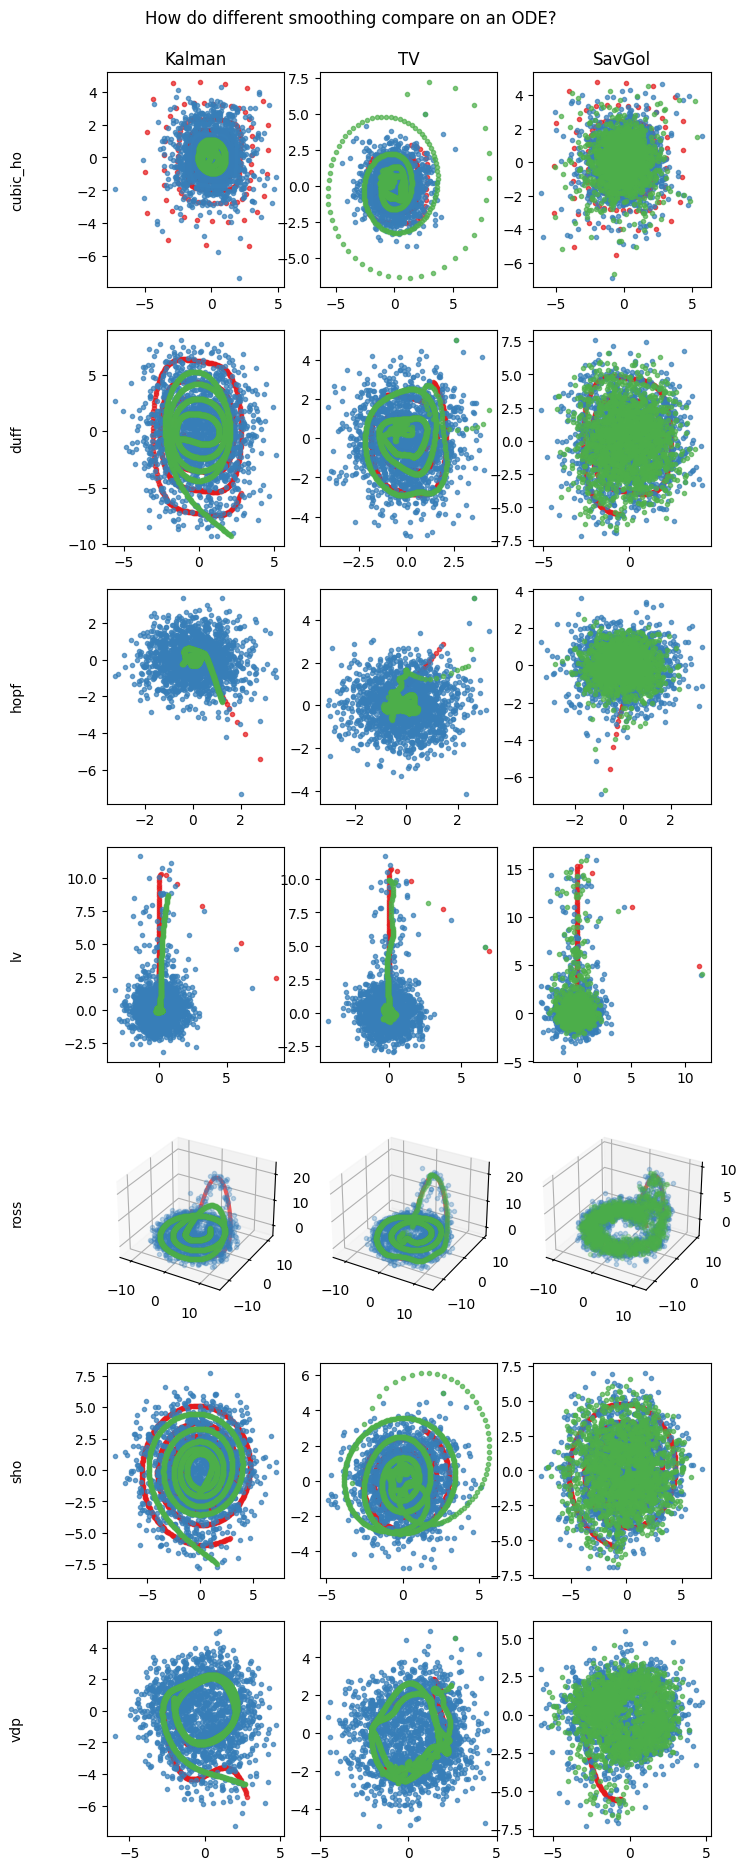
\includegraphics[width=\textwidth]{images/summary_train}
\end{figure}
\begin{figure}
    \label{fig:test}
    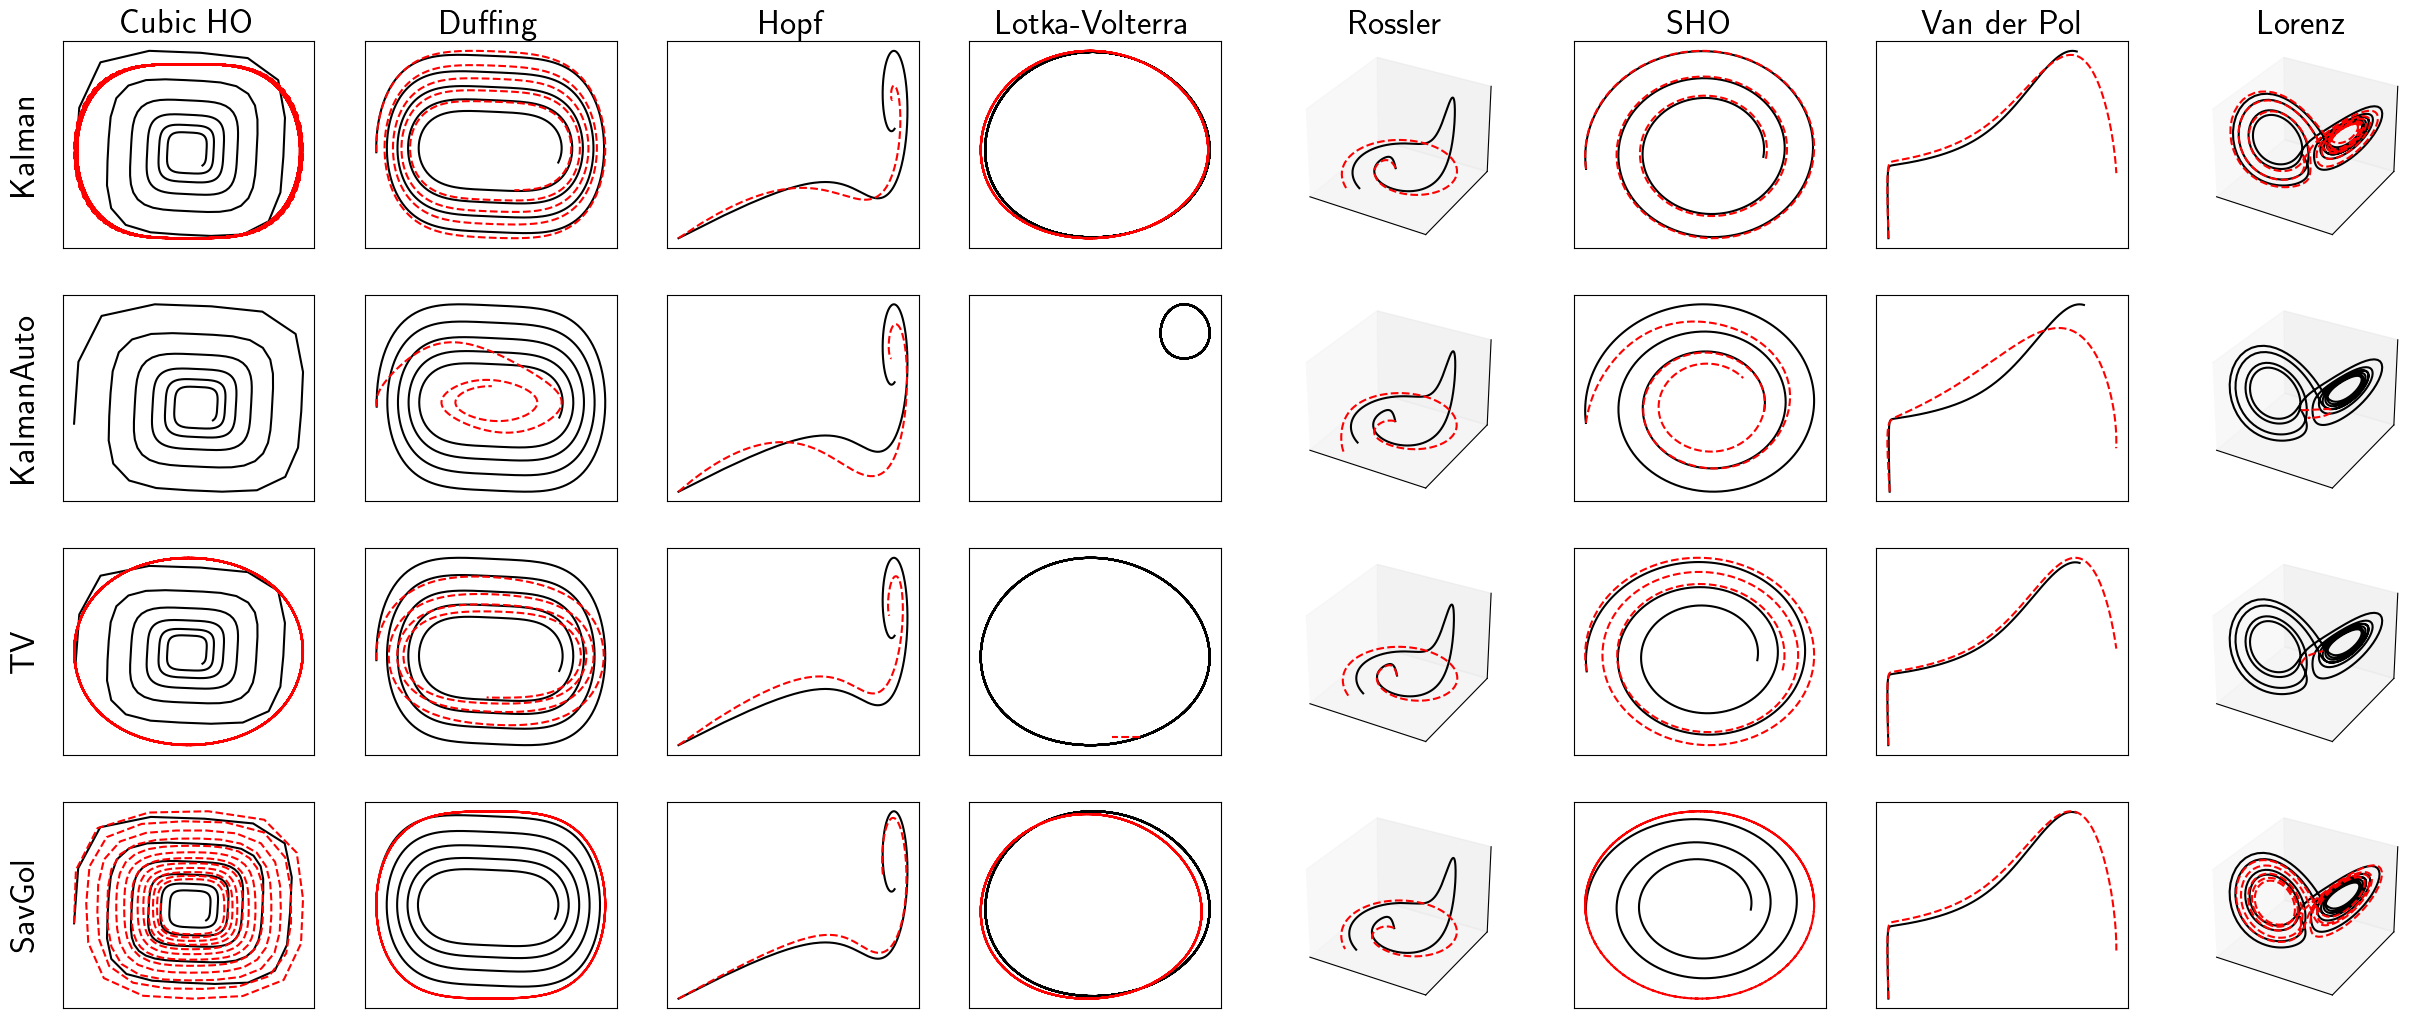
\includegraphics[width=\textwidth]{images/summary_test}
\end{figure}
\begin{figure}
    \label{fig:f1}
    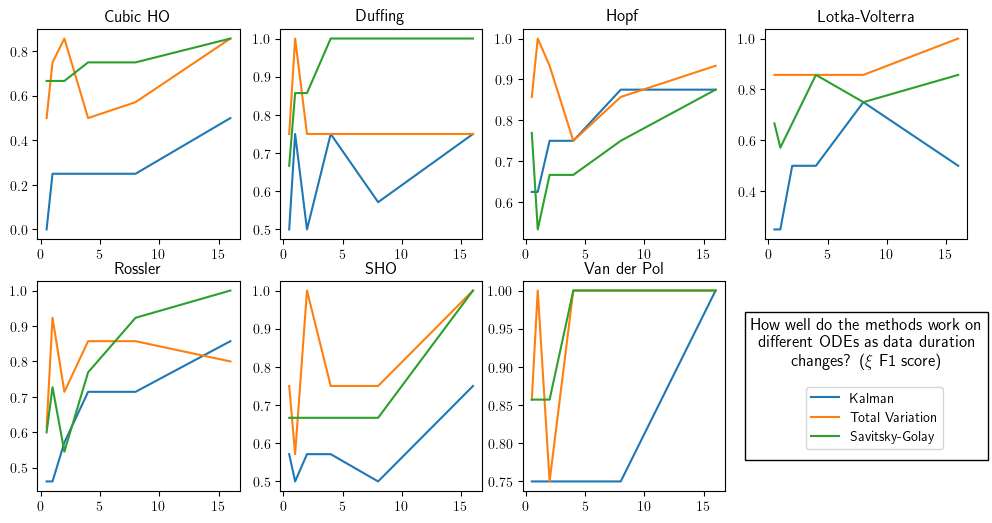
\includegraphics[width=\textwidth]{images/summary_f1}
\end{figure}
\begin{figure}
    \label{fig:mae}
    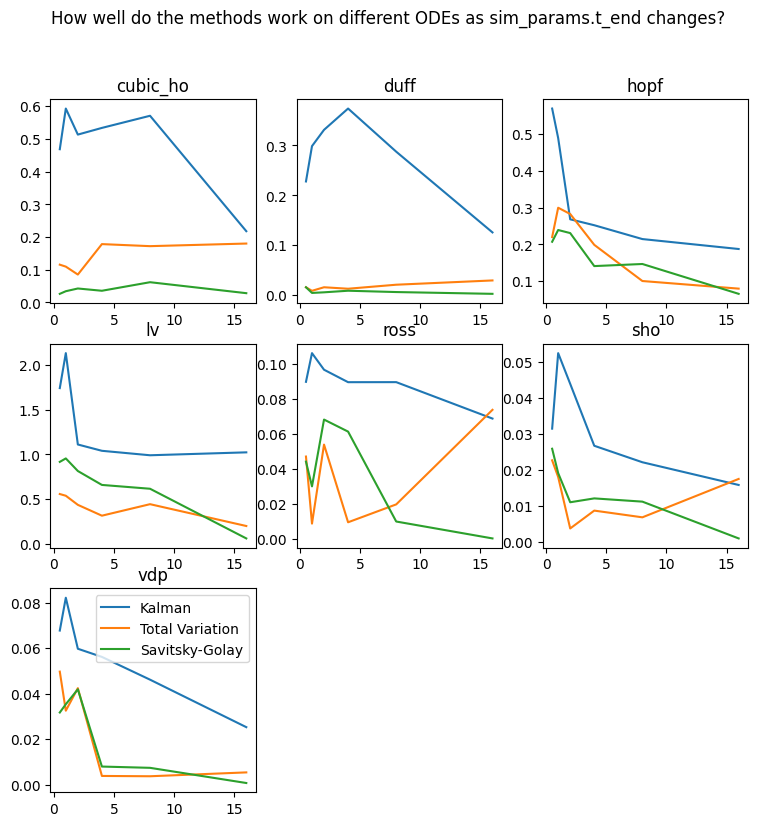
\includegraphics[width=\textwidth]{images/summary_mae}
\end{figure}
% Methods:
% \begin{itemize}
%     \item table
%     \item Compare with (a) WeakSINDy, (b) TV, SG filter
%     \item metrics: F1, MAE of coefficients (\textcolor{red}{or MSE?})
%     \item Utilize MIOSR optimizer (\textcolor{red}{with Ensembling wrapper?})
% \end{itemize}
% ODE data sets \textcolor{red}{Do I add {\it all} the possible ones I have set up (Rossler, Duffing)?  Do I add the reaction network one?}
% \begin{itemize}
%     \item Hudson Bay Company Lotka-Volterra
%     \item Van der Pol oscillator
%     \item Hopf
%     \item MHD \textcolor{red}{Would need to add}
% \end{itemize}
% PDE Data sets \textcolor{red}{anything real?}
% \begin{itemize}
%     \item Inviscid Burgers
%     \item KdV
%     \item nonlinear Schrodinger
%     \item KS
%     \item Reaction-Diffusion
% \end{itemize}

% \subsection{Noise tolerance and data length}
% \textcolor{blue}{Figure: plot of score for each method across range of smoothing parameters.  subplots for each ODE \& metric}.  \textcolor{red}{Parameter-search wrapper-experiment inside P-search comparison experiment}.
% % \subsection{ODEs: Robust Kalman Smoothing (Maybe?)}
% \textcolor{blue}{Figure: plot of score for each method across range of smoothing parameters.  subplots for each ODE \& metric}.
% Add noisy
% \subsection{ODEs: Data Length requirements}
% \textcolor{blue}{Figure: plot of score for each method at optimal parameter across range of data length requirements.  subplots for each ODE \& metric}.  \textcolor{red}{Parameter-search wrapper-experiment inside data-length wrapper-experiment inside Data-length comparison comparison experiment}.
% \subsection{PDEs}
% \textcolor{red}{Use Figure 4 from the E-SINDy paper. Need to implement these}
% % \subsection{Model Predictive Control}
% % \textcolor{red}{Lorenz stabilization, learn from E-SINDy paper}
\section{Conclusion}
\green{TBD}
This paper has demonstrated that Kalman smoothing is a useful addition to SINDy.  By incorporating hyperparameter optimization, it makes the method more generally applicable across domains. The Kalman smoother behaves optimally for the simplest systems and provides a familiar process to the controls engineering community, even if it is not a mathematically unique innovation.  It also appears to perform better at preserving global system structure in simulation.

<More specific experimental results summary>

Since Kalman smoothing and SINDy regression loss terms accomodate variable timesteps, a natural innovation is to combinine the two into a single optimization problem.  \cite{Hirsh2022} were the first to do so.  This could allow interaction and a more clear tradeoff between fitting the data through either the smoothed process or the coefficient sparsity.

Currently, the hyperparameter optimization has no access to the terms in the SINDy expression and therefore no intrinsic understanding of the process variance even when measurement noise is known.  With access however to the library terms, hyperparameters for process and measurement variance could be more quickly selected, rather than the long prox-gradient method of \cite{Barratt2020}.

Kalman SINDy could also be more directly compared to Weak SINDy, which aims at the same goal of reducing the sensitivity to noise.

Oh wait, did I forget to mention that KS has a natural connection between

\section*{Appendix}
\begin{table}[ht]
    \centering
    \label{tab:ODEs}
    \begin{tabular}{c c c}
        System & ODE & Experiment parameters\\
        \hline\hline
        Linear Damped Oscillator
            & $\dot {\vec x} = \left[\begin{matrix}-\alpha & \beta \\ -\beta & -\alpha\end{matrix}\right] \vec x$
            & $\alpha = .1$, $\beta=2 $\\\\
        Cubic Damped Oscillator
            & $\dot {\vec x} = \left[\begin{matrix}-\alpha & \beta \\ -\beta & -\alpha\end{matrix}\right] \left[\begin{matrix}x_1^3\\x_2^3\end{matrix}\right]$
            & $\alpha = .1$, $\beta=2 $\\\\
        Duffing
            & $\dot {\vec x} = \left[\begin{matrix}x_2 \\ -\alpha x_2 - \beta x_1 -\gamma x_1^3\end{matrix}\right]$
            & $\alpha = .2$, $\beta=.05 $, $\gamma=1$\\\\
        Hopf
            & $\dot {\vec x} = \left[\begin{matrix}
                -\alpha x_1 -\beta x_2 - \gamma x_1(x_1 ^2 + x_2^2) \\
                \beta x_1 - \alpha x_2 -\gamma x_2(x_1 ^2 + x_2^2)
            \end{matrix}\right]$
            & $\alpha = .05$, $\beta=1 $, $\gamma=1$\\\\
        Lotka-Volterra
            & $\dot {\vec x} = \left[\begin{matrix}
                \alpha x_1 - \beta x_1 x_2 \\
                \beta x_1  x_2 - 2 \alpha x_2
            \end{matrix}\right]$
            & $\alpha = TBD$, $\beta=TBD $\\\\
        Rossler
            & $\dot {\vec x} = \left[\begin{matrix}
                -x_2 - x_3 \\
                x_1 + \alpha x_2\\
                \beta + (x_1 - \gamma) x_3
            \end{matrix}\right]$
            & $\alpha = .2$, $\beta=.2 $, $\gamma=5.7$\\\\
        Van der Pol Oscillator
            & $\dot {\vec x} = \left[\begin{matrix}
                x_2 \\
                \alpha(1 - x_1^2) x_2 - x_1
            \end{matrix}\right]$
        & $\alpha = .5$
    \end{tabular}
    \caption{The parametrization of ODEs used in these experiments.  Mostly from defaults in the pysindy package.}
\end{table}

\begin{table}
    \label{tab:exp-params}
    \begin{tabular}{c c c}
        Parameter & Symbol & value\\
        \hline
    \end{tabular}
\end{table}


\bibliography{main}
\end{document}
